%========================================
\chapter{Results}
%========================================

\section{Implementation Achievements}
\begin{itemize}
  \item 24 frontend React page components across three portals (Farmer, Staff, Admin).
  \item 18+ REST API endpoints organized in 9 domain-specific routers, all operational.
  \item Real-time SSE queue stream delivering updates every 5 seconds.
  \item ML wait time predictor with R\textsuperscript{2}~=~0.988 integrated at booking and queue.
  \item Complete procurement verification workflow with quality grading.
  \item Full payment lifecycle: Scheduled $\to$ Processing $\to$ Settled with disputes.
  \item Web Push Notifications delivered to farmer browsers via VAPID.
  \item AI Command Agent (LangChain + Gemini) for natural language system queries.
\end{itemize}

\section{Screenshots of Working Modules}

The AgriQueue web application was deployed and validated across end-to-end user workflows spanning the public discovery portal, authenticated farmer management, interactive slot reservation, token issuance, live SSE queue tracking, and procurement center staff counter operations. Figures~\ref{fig:ss-home} through~\ref{fig:ss-staff} illustrate key working modules of the live application.

\clearpage

\begin{figure}[H]
  \centering
  \fboxsep=0pt\relax
  {\color{gray!40}\fbox{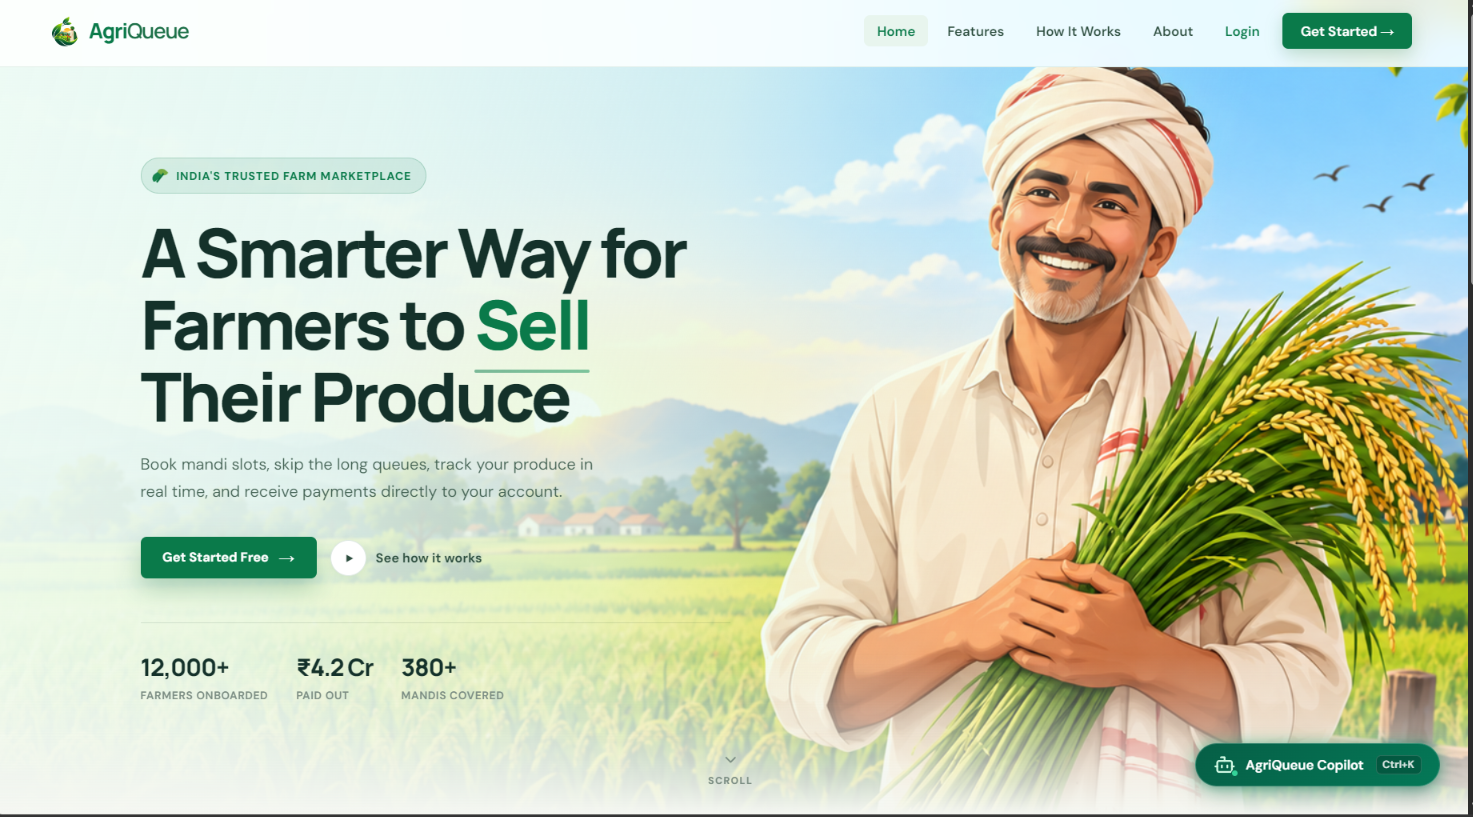
\includegraphics[width=0.86\textwidth]{img/screenshot_home.png}}}
  \caption{AgriQueue Public Landing Page and Discovery Portal}
  \label{fig:ss-home}
  \vspace{0.6cm}
  {\color{gray!40}\fbox{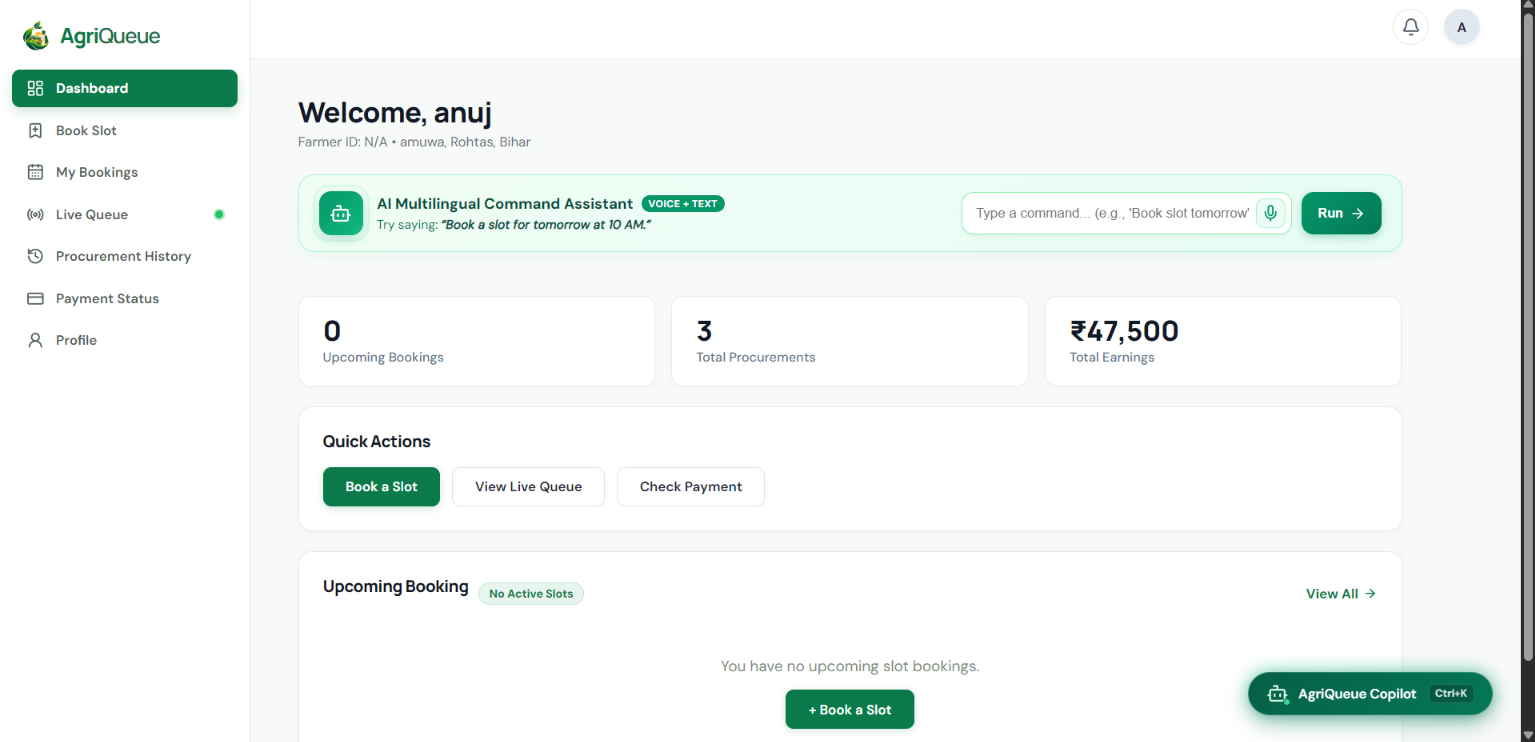
\includegraphics[width=0.86\textwidth]{img/screenshot_farmer_dashboard.png}}}
  \caption{Farmer Dashboard with KPI Summary and AI Multilingual Assistant}
  \label{fig:ss-dash}
\end{figure}
\clearpage

\begin{figure}[H]
  \centering
  \fboxsep=0pt\relax
  {\color{gray!40}\fbox{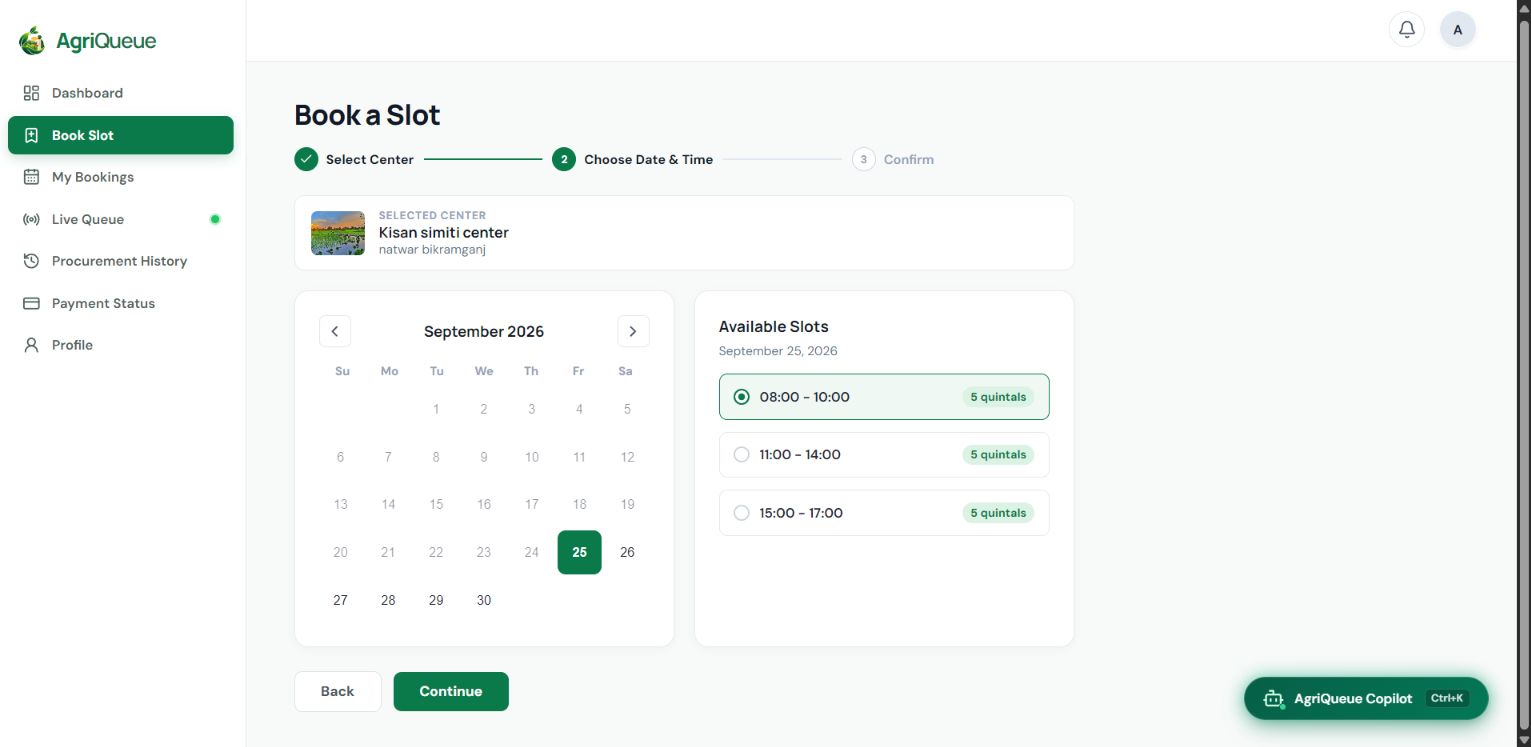
\includegraphics[width=0.86\textwidth]{img/screenshot_book_slot.png}}}
  \caption{Slot Booking Workflow with Interactive Calendar and Slot Capacity}
  \label{fig:ss-book}
  \vspace{0.6cm}
  {\color{gray!40}\fbox{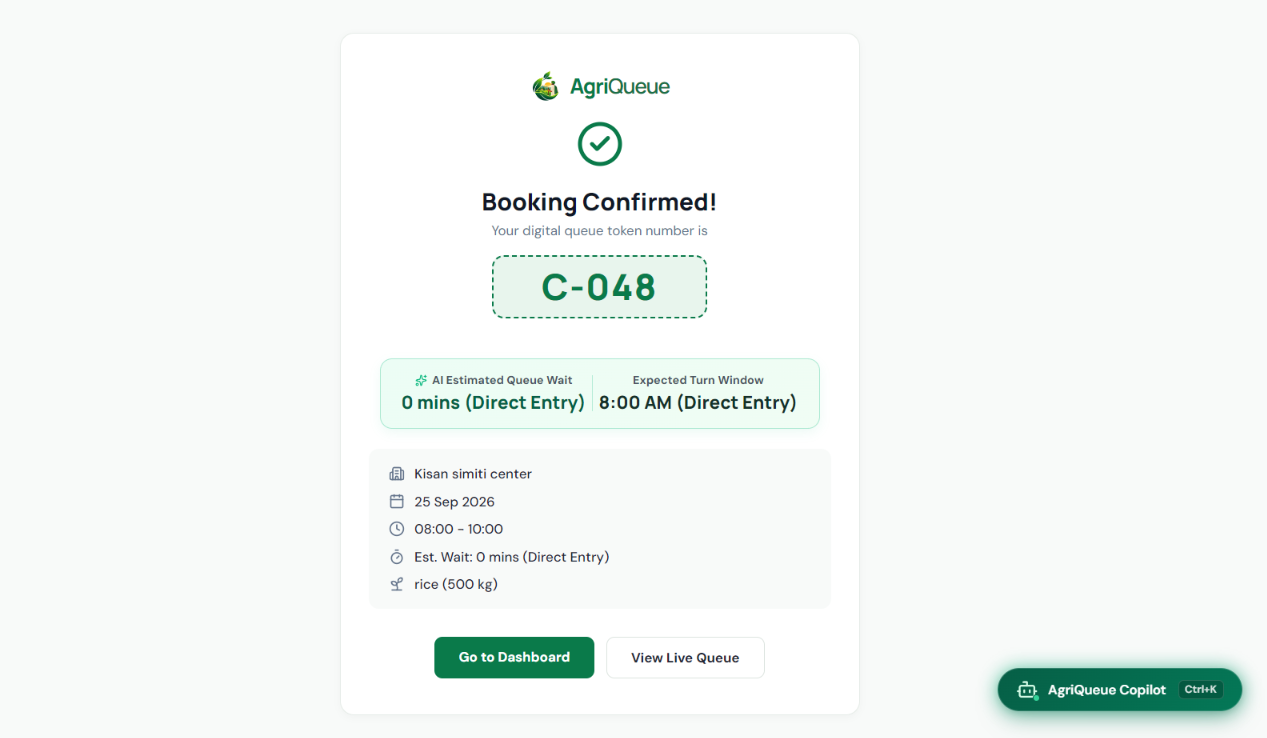
\includegraphics[width=0.86\textwidth]{img/screenshot_booking_confirmed.png}}}
  \caption{Booking Confirmation with Token Issuance (C-048) and AI Wait Estimate}
  \label{fig:ss-confirm}
\end{figure}
\clearpage

\begin{figure}[H]
  \centering
  \fboxsep=0pt\relax
  {\color{gray!40}\fbox{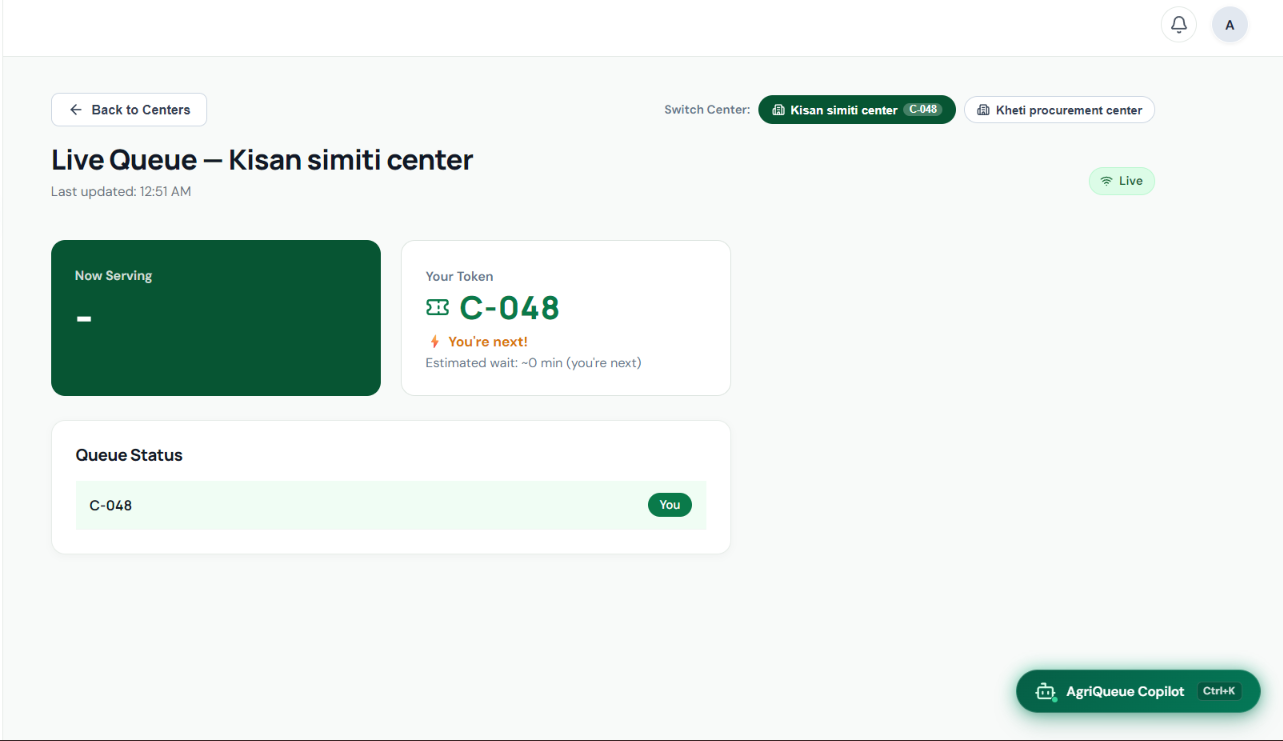
\includegraphics[width=0.86\textwidth]{img/screenshot_live_queue.png}}}
  \caption{Farmer Live Queue Real-Time Tracking Interface}
  \label{fig:ss-queue}
  \vspace{0.6cm}
  {\color{gray!40}\fbox{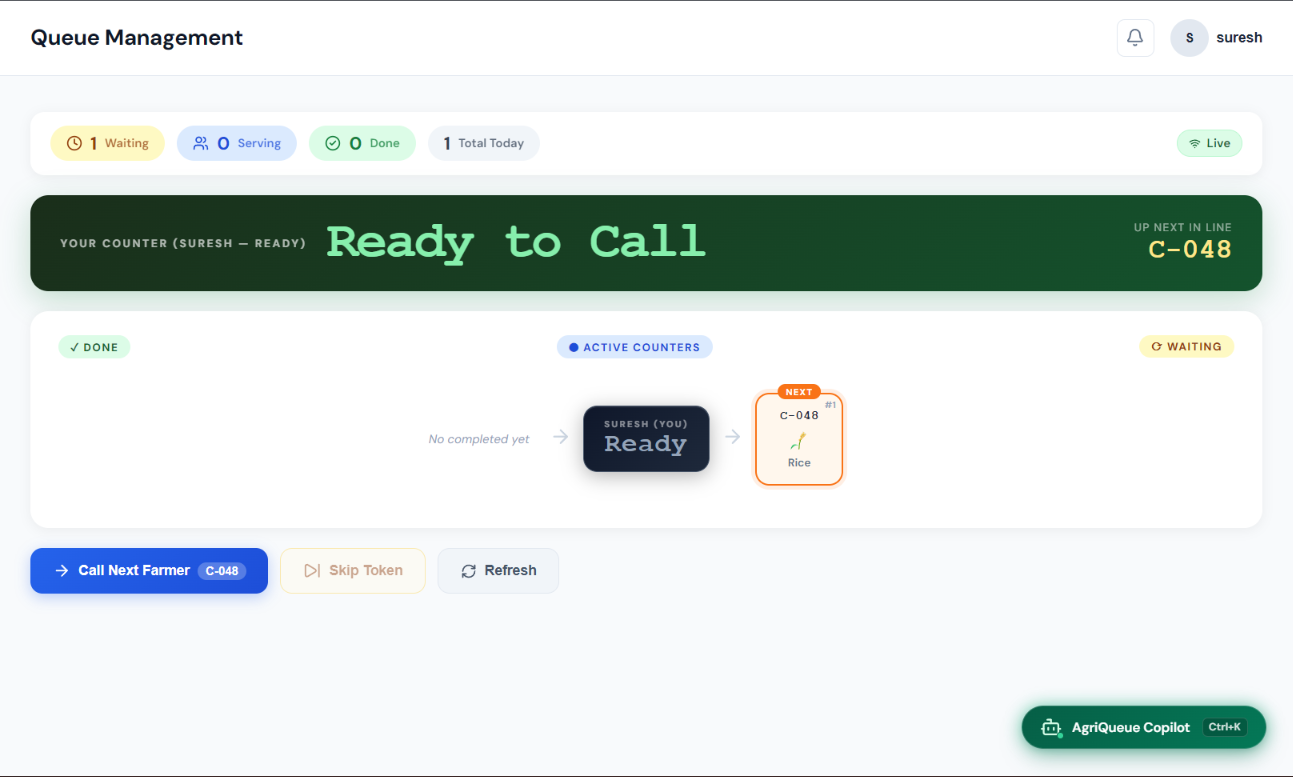
\includegraphics[width=0.86\textwidth]{img/screenshot_staff_queue.png}}}
  \caption{Staff Queue Management Console with Active Counter Workflow}
  \label{fig:ss-staff}
\end{figure}
\clearpage

\section{ML Prediction Sample Results}

\begin{table}[h!]
\centering
\caption{ML Wait Time Prediction Samples}
\label{tab:ml-samples}
\renewcommand{\arraystretch}{1.2}
\begin{tabular}{|p{1.8cm}|p{1.4cm}|p{1.8cm}|p{2.2cm}|p{2.6cm}|p{2.8cm}|}
\hline
\textbf{Crop} & \textbf{Ahead} & \textbf{Qty (kg)} & \textbf{Slot} & \textbf{Predicted} & \textbf{Congestion} \\ \hline
Wheat & 0 & 1000 & 10:00 AM & 0 min (Direct) & No Wait \\ \hline
Paddy & 3 & 800  & 10:00 AM & 28 min & Low Wait \\ \hline
Wheat & 5 & 1000 & 10:00 AM & 47 min & Moderate \\ \hline
Cotton & 8 & 1500 & 11:00 AM & 72 min & High Demand \\ \hline
Mustard & 12 & 2000 & 09:00 AM & 108 min & Peak Congestion \\ \hline
Maize & 2 & 500 & 01:00 PM & 19 min & Low Wait \\ \hline
\end{tabular}
\end{table}

\section{Outputs and Observations}
\begin{itemize}
  \item \textbf{Farmer:} Slot booked with unique token (e.g., ``C-048'') in 3 API calls. SSE queue updates every 5 seconds in browser.
  \item \textbf{Staff:} Calling a token updates status to ``Serving'' and all SSE clients refresh immediately.
  \item \textbf{Procurement:} Net payable computed as: \texttt{(actual\_weight - deductions) \texttimes\ rate\_per\_kg}.
  \item \textbf{Payment:} Receipt number auto-generated as \texttt{RCP-XXXXXX}; expected settlement date = booking\_date + 2 days.
  \item \textbf{Admin:} Center IDs auto-start at 1000 (via PostgreSQL Sequence). All metrics refresh in real-time.
\end{itemize}
